\documentclass{ximera}

\author{Bart Snapp}

\title{Torus and circles}

\begin{document}
\begin{abstract}
  One group member will plot a torus with two circles on it.
\end{abstract}
\maketitle

One group member will produce a plot like this one:
\begin{image}
  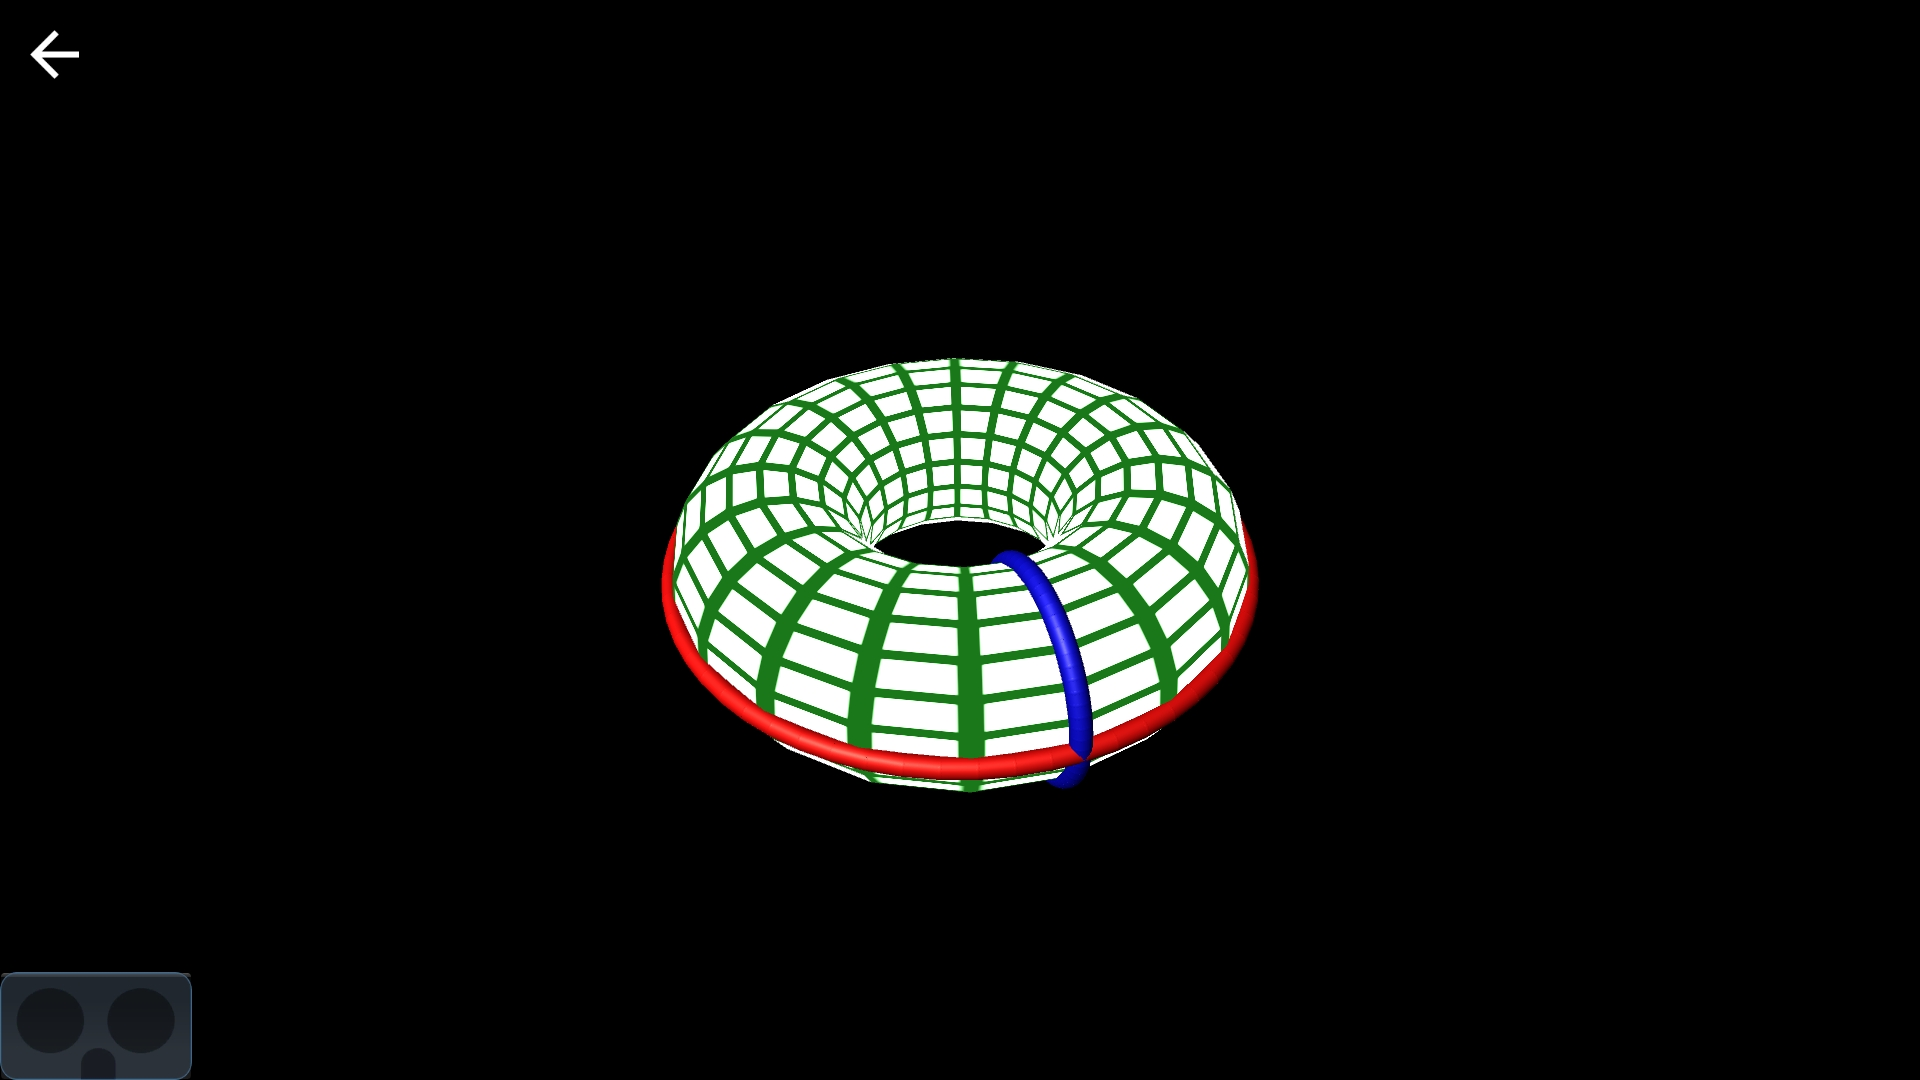
\includegraphics{torusAndCircles.png}
\end{image}

This is a torus with two circles on it where the radius from the
center of the torus to the center of the tube is $2$, and the radius
of the tube is $1$.


As a gesture of friendship, I will tell you that the parametric
formula for a torus of radius $R$ is:
\begin{align*}
  x(s,t) &= (R + r\cdot \cos(t))\cos(s)\\
  y(s,t) &= (R + r\cdot \cos(t))\sin(s)\\
  z(s,t) &= r\cdot \sin(t)
\end{align*}
where $R$ is the radius from the center of the torus to the center
of the tube, and $r$ is the radius of the tube.

  
You may color you circles any color you like---though you must make
them \textbf{different} colors.
\end{document}
